% Copyright (c) 2005-2008 Center for Urban Simulation and Policy Analysis,
% University of Washington.  Permission is granted to copy, distribute and/or
% modify this document under the terms of the GNU Free Documentation License,
% Version 1.2 or any later version published by the Free Software Foundation;
% with no Invariant Sections, no Front-Cover Texts, and no Back-Cover Texts.
% A copy of the license is included in the section entitled "GNU Free
% Documentation License".

\chapter{Installation}
\label{chapter:installation}

\index{installation}

\section{Installing OPUS}
OPUS runs on any platform that Python runs on, such as Windows, Linux and OS X.  Instructions for installing OPUS, and UrbanSim, which is bundled with it. are maintained online at www.urbansim.org.  For users with a computer running Windows, it is recommended to install the \emph{Latest Development Version}, using the Windows Installer downloadable from http://www.urbansim.org/opus/installer/opus\_installer.exe.  Step by step details for using the installer are available at http://www.urbansim.org/docs/installation.  Follow these instructions on the web for the installation, and return to this document for the following tests of the install.  Please note that the installer actually launches other installers for supporting packages during the install process, and that you need to be connected to the Internet for the installer to download files during the installation (please be patient - the installation takes 20-30 minutes depending on your connection speed).

The software is being continuously developed and refined, with bug fixes and new features being added.  In order to get these updates, or to download and install other OPUS Packages not initially installed, users will need an application that can retrieve updates and packages from the Subversion repository for the software.  Subversion is a version control system used by many software development projects, and there are many free software tools available for accessing it.  One of these, on the Windows platform, is Tortoisesvn, available from http://tortoisesvn.tigris.org/.  Users can download and install this package, and it will extend the Windows Explorer file browser, allowing packages to be \emph{checked out} of the repository (downloaded for the first time), or \emph{updated} if they have already been checked out previously.  Subversion compares the version on your local machine with the version on the server, and if there is a newer version of any component, it will download it and replace the version on your machine with the most current one available.

To check out (download for the first time) any package from the OPUS repository, if you have installed Tortoisesvn, right-click on the opus/src folder in the Windows Explorer, and the menu will contain new entries for interacting with Subversion.  Select the \verb#SVN Checkout# option, and use the URL: \verb#https://trondheim.cs.washington.edu/svn/opus/trunk#, plus the name of any package you wish to check out.  The target local directory should be under the OPUS\_HOME/src directory, and take the same name as the OPUS Package you are checking out.  An example of this checkout dialog is shown in Figure \ref{fig:tortoisesvn}.  There are other Subversion clients available for Windows, OS X and Linux, and any of them should work equivalently well for obtaining OPUS packages.  Eventually, this functionality may be embedded into the OPUS GUI.

\begin{figure}[htp]
\begin{center}
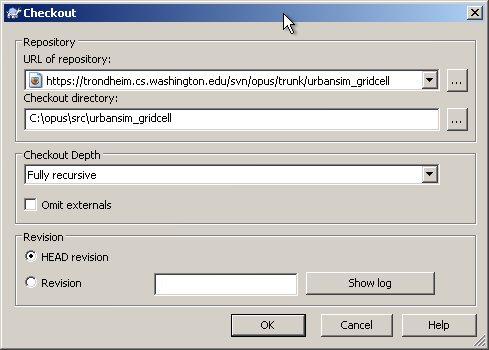
\includegraphics[scale=0.4]{graphics/tortoisesvn.png}
\end{center}
\caption{Checking Out a Package using the TortoiseSVN Subversion Client}
\label{fig:tortoisesvn}
\end{figure}

Once a user makes changes on their local machine to any content that has been checked out from the repository, the changed file will be inconsistent with the version in the repository.  In many cases, this is fine, but if the file is updated by someone else and checked into the repository, then the next time you update from the repository, you will have conflicting changes in the file you have modified.  There are tools available to reconcile the conflicts, but the best approach for most users is to isolate the places you want to make changes to a location that will not have collisions with ongoing updates in the repository.  A project\_configs directory is intended for users to create and manage their own projects.  If the user needs to modify Python modules within the various OPUS packages, these can most easily be handled by creating another OPUS package of your own that \emph{inherits} from the package you want to change, and contains only the modified versions of files.   Note that OPUS packages can be updated from the repository at any time by selecting the directory (or all of them at once), right-clicking, and selecting the menu item for \verb#SVN Update#.

Once OPUS is installed, it is a good idea to test whether it is installed correctly.  Since the installation involves downloading and installing numerous components (all managed easily by the Windows installer), there are times when a component does not download properly and fails to install.  Here are a few simple tests to ensure that Python and the key libraries were properly installed.

\begin{enumerate}
\item Start a command window or shell (on Windows, this can be done from the start menu \verb#run# and entering \verb#cmd#.
\item Type \verb#python# and press Enter (for brevity, I will not repeat the press Enter at the end of each command - it is implied).  A Python prompt should appear, as \verb#>>>#.
\item Type \verb#import numpy#.  It should just generate another Python prompt, which means it successfully imported the Numpy library.  If it fails, you will see an errror, and need to exit Python and reinstall Numpy.  To see what version of Numpy is installed, type \verb#print numpy.__version__#.
\item Repeat the import step with the following libraries: scipy, matplotlib, sqlalchemy, and PyQt4 (the capitalization matters).  If all of these import without reporting an error, the main libraries are installed correctly.  The version number for sqlalchemy should be at least 0.4.3 at the time of this writing.
\end{enumerate}

To exit an interactive Python session, you can type Control-Z, or quit().  Please exit Python before proceeding.

\section{The OPUS Graphical User Interface}
A new Graphical User Interface (GUI) is in development at this time.  A working version is available, but it will continue to evolve very rapidly over the next several months, at least.  Screenshots and descriptions in this section will need to be revised relatively soon to reflect these changes.

\subsection{Launching the OPUS GUI}
To launch, or run, the OPUS GUI, you will need to run a python script called opus.py in the /opus/src/opus\_gui directory\footnote{Note the use of forward slashes in the path.  On most operating systems, and in Python, forward slashes are used to indicate separations in the path components.  On Windows, backward slashes are used instead.  Python can actually use forward slashes and translate them appropriately on Windows or other operating systems as needed, so we will use the convention of forward slashes throughout the text, for generality.}.  If you have used the Windows installer to install OPUS, then a Windows \verb#Start# menu item has been added under the Opus menu item under programs, so launching OPUS is a simple as selecting the \verb#OpusGUI Opus# menu item.  If you did not use the installer, for example, on OS X, or Linux, then open a command window or shell, change directory to the opus\_gui directory and type \verb#python opus.py#.  In Windows, you can also double-click on the opus.py file in the /opus/src/opus\_gui directory to launch the GUI.

However it is launched, it will start from a command shell, and this window remains active while OPUS is running.  Do not attempt to quit this window or OPUS will close also.  After launching OPUS, the main OPUS GUI window should be displayed as in Figure \ref{fig:opus1}.

\begin{figure}[htp]
\begin{center}
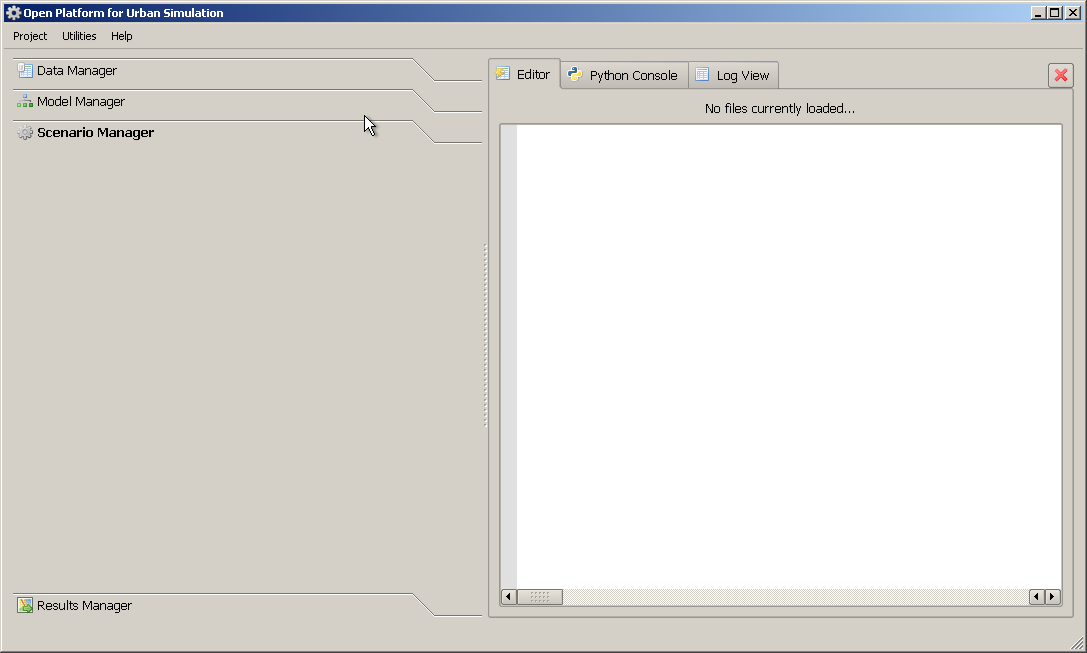
\includegraphics[scale=0.4]{graphics/opus1.png}
\end{center}
\caption{OPUS GUI Main Window}
\label{fig:opus1}
\end{figure}

The main window contains a section on the left with four tabs in it, labeled \emph{Data Manager}, \emph{Model Manager}, \emph{Scenario Manager}, and \emph{Results Manager}.  Each tab provides a location for configuring and running a variety of tasks, organized into the main functional areas involved in developing and using a simulation model.  

\squishlist
\item The \emph{Data Manager} organizes the processes related to moving data between the OPUS environment and, doing data processing both within OPUS, and also remotely in a database or GIS environment.  OPUS can use Python to pass data and commands to a database system like Postgres or MS SQL Server, or to a GIS system like ArcGIS or PostGIS.  Tasks can be organized in the Data Manager as scripts, and run as a batch, or alternatively, they may be run interactively.
\item The \emph{Model Manager} organizes the work of developing, configuring, and estimating the parameters of models, and of combining models into a model system.
\item The \emph{Scenario Manager} organizes the tasks related to configuring a scenario of input assumptions, and to interact with a run management system to actually run simulations on scenarios.  Tools to monitor and interact with a running simulation are provided here.
\item The \emph{Results Manager} provides the tools to explore results once one or more scenarios have been simulated.  It integrates an Indicator Framework that makes it possible to generate a variety of indicators, for diagnostic and for evaluation purposes.  It also provides functionality to visualize indicators as charts, maps, and tables, and to export results to other formats for use outside of OPUS.
\squishend

Notice that at this point there are no contents in any of the four tabs.  OPUS uses a novel approach to dynamically creating and managing content in the GUI by loading, editing, and saving content in the form of XML files.  XML stands for Extensible Markup Language, and is an extension of the HTML markup language used to display web pages.  It is more flexible, and has become widely used to store content in a strucured form.  

To add content to the GUI, we will load a \emph{Project}, which is in fact, just an XML file containing configuration information.  From the main menu, load a project from eugene\_gridcell.xml, which is in the default location of opus/project\_configs.  The OPUS window should now appear as in Figure \ref{fig:opus2}.

\begin{figure}[htp]
\begin{center}
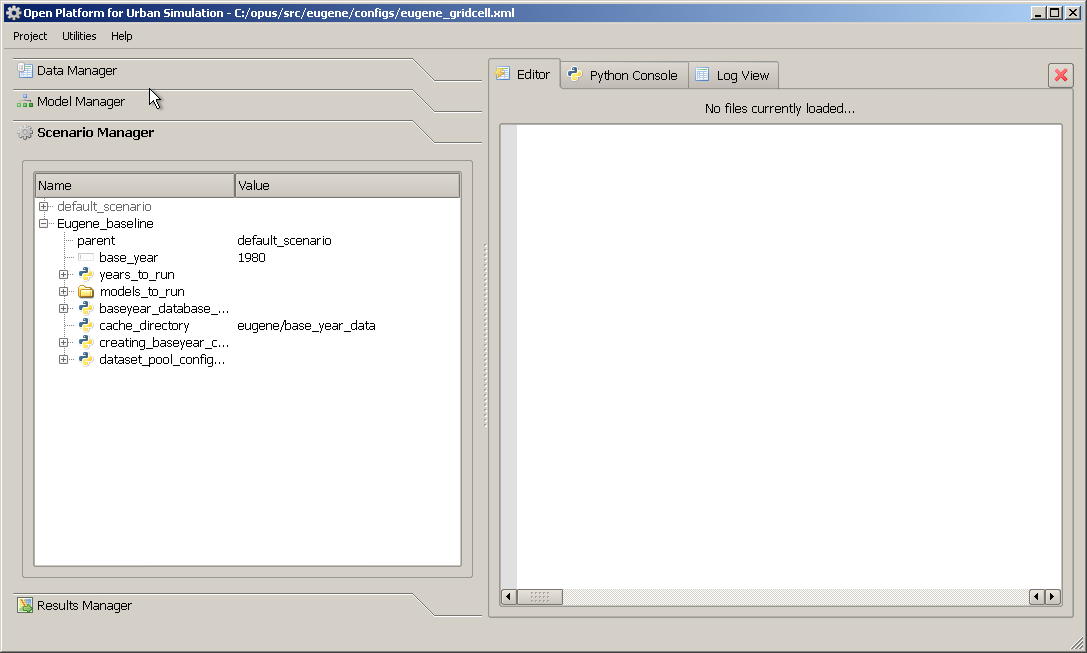
\includegraphics[scale=0.4]{graphics/opus2.png}
\end{center}
\caption{OPUS GUI Main Window}
\label{fig:opus2}
\end{figure}

A small section of the eugene\_gridcell.xml file is shown in Figure \ref{fig:opus-xml}.  It is just text, but in a structured format, with nodes corresponding to information that is displayed in the GUI.  Some of the content of the XML provide data used by the GUI to determine how to display information, or what menu items are appropriate to connect to the node in the GUI.

\begin{figure}[htp]
\begin{center}
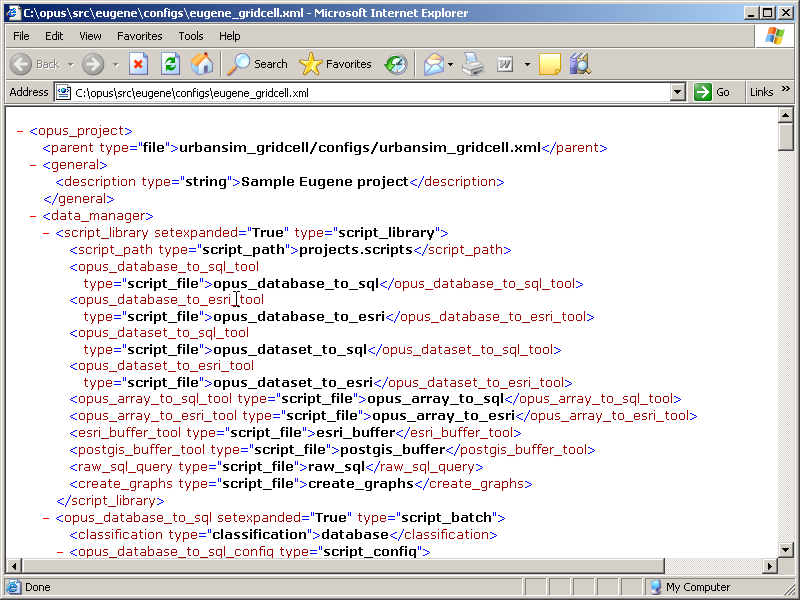
\includegraphics[scale=0.4]{graphics/opus-xml.png}
\end{center}
\caption{An Excerpt from eugene$\_$gridcell.xml}
\label{fig:opus-xml}
\end{figure}

Note that one of the first entries in the xml file is a \emph{parent} type, and that this line refers to another xml file named urbansim/gridcell.xml.  This reflects an important aspect of the GUI design: it supports inheritance among projects.  In practical terms for a user, this means that you can use default projects as templates, or parents, for another project you want to create that is mostly the same as an existing project, but has some changes from it.  The new project is called a \emph{child} project, and it inherits all of its information from the \emph{parent}, but can override any aspect it so chooses from the parent.  The parallels with human behavior are pretty obvious!

Users will create their own projects in the opus/project\_configs directory.  This will allow them to keep projects localized in one place, and to avoid editing and possibly corrupting one of the projects that are in an OPUS package.

\section{A Test Drive}
\subsection{Running a Simulation}
Once a project has been developed, including the data to be used in it, and the model system has been configured and the parameters for the models estimated, the next step is to create and run a scenario.  In the eugene\_gridcell project, a baseline scenario has already been created and is ready to run.  To run this scenario, in the Scenario Manager, right-click with the mouse on the Eugene-baseline entry and select \verb#Run this Scenario#.  At this point, a frame should appear in the right hand side of the OPUS window, as shown in Figure \ref{fig:opus-start-run}.

\begin{figure}[htp]
\begin{center}
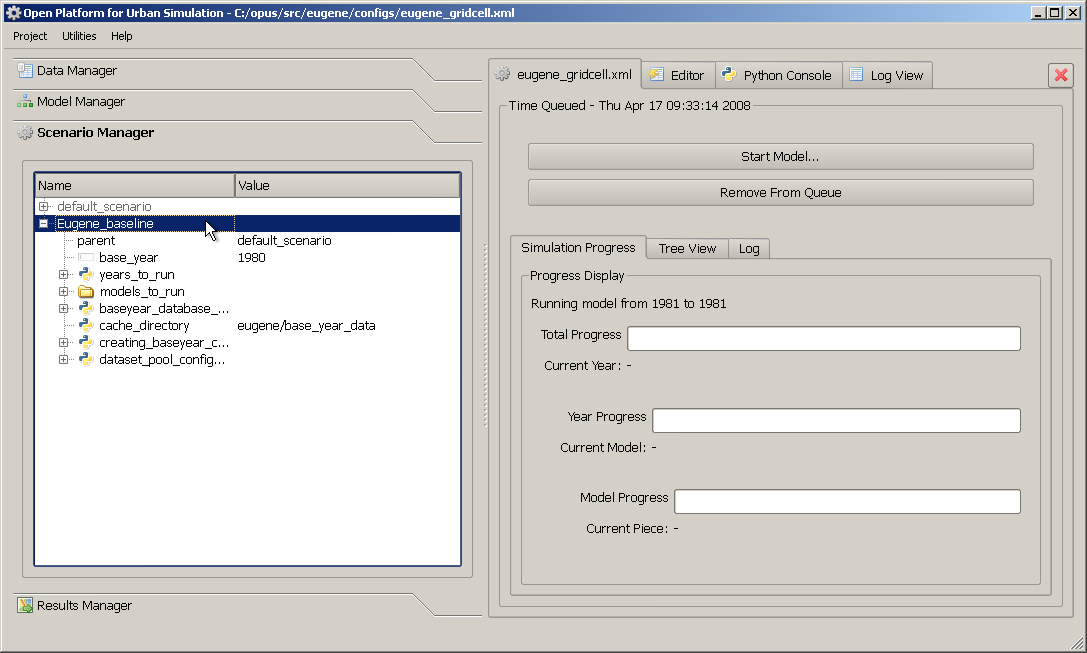
\includegraphics[scale=0.4]{graphics/opus-start-run.png}
\end{center}
\caption{Starting a Simulation on a Scenario.xml}
\label{fig:opus-start-run}
\end{figure}

The frame on the right contains an option to start the run and an option to remove the run from the queue.  The latter will remove this new frame so that it is no longer available to run.  Start the run with the first button option, labelled \verb#Start Model#.  The window will now update as the simulation proceeds, with progress bars and labels being updated to show the changing state of the system, such as what year the model is simulating, what model is running, and even what part of a model is running.  Figure \ref{fig:opus-running} shows the updated window in this state.  Note that the \verb#Start Model#  button label has now changed to \verb#Pause Model#.  If this is pressed while the model system is running, a request to pause the model is triggered, and once the current model in the model system is finished, the system pauses until you take further action, like resume, or remove from queue.

\begin{figure}[htp]
\begin{center}
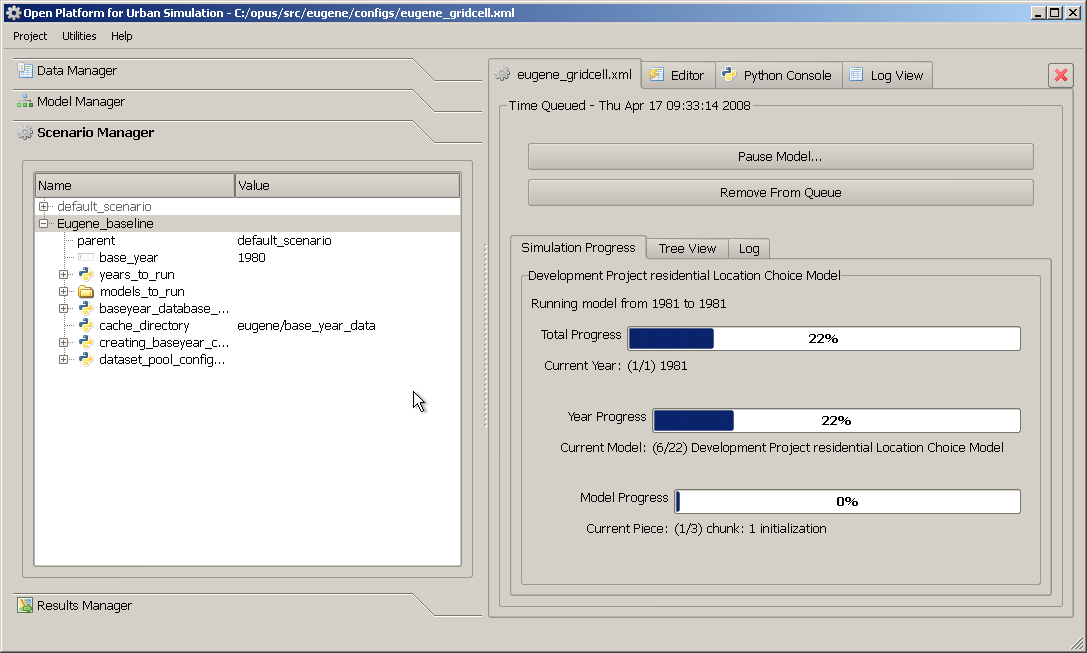
\includegraphics[scale=0.4]{graphics/opus-running.png}
\end{center}
\caption{Running a Simulation on a Scenario.xml}
\label{fig:opus-running}
\end{figure}

\subsection{Generating Indicators}
Once the simulation is finished, which should not take long since the initial configuration only runs for one year, you can explore the results in the Results Manager.  Click on the Results Manager tab, and expand the model.gridcell entry under Indicator\_libraries.You will see some initial indicators that are available.  Right-click on the population indicator and select \emph{Generate results with}.  The screen should now show a new frame on the right that has pull-down menus to configure and compute this indicator, shown in Figure \ref{fig:opus-generate-indicator}.  The initial indicator is a population by gridcell indicator, which requires computing the number of persons in each household that are located in buildings that are located in gridcells.  This particular example uses a variable to do this computation.  Variables are coded as very small Python programs.  An alternative, simpler approach to use is the OPUS Expression Language, which has been recently created to make available to non-programmers much of the power of doing complex calculations such as this, with a simple syntax.  This is covered in the documentation, and later in this chapter. 

\begin{figure}[htp]
\begin{center}
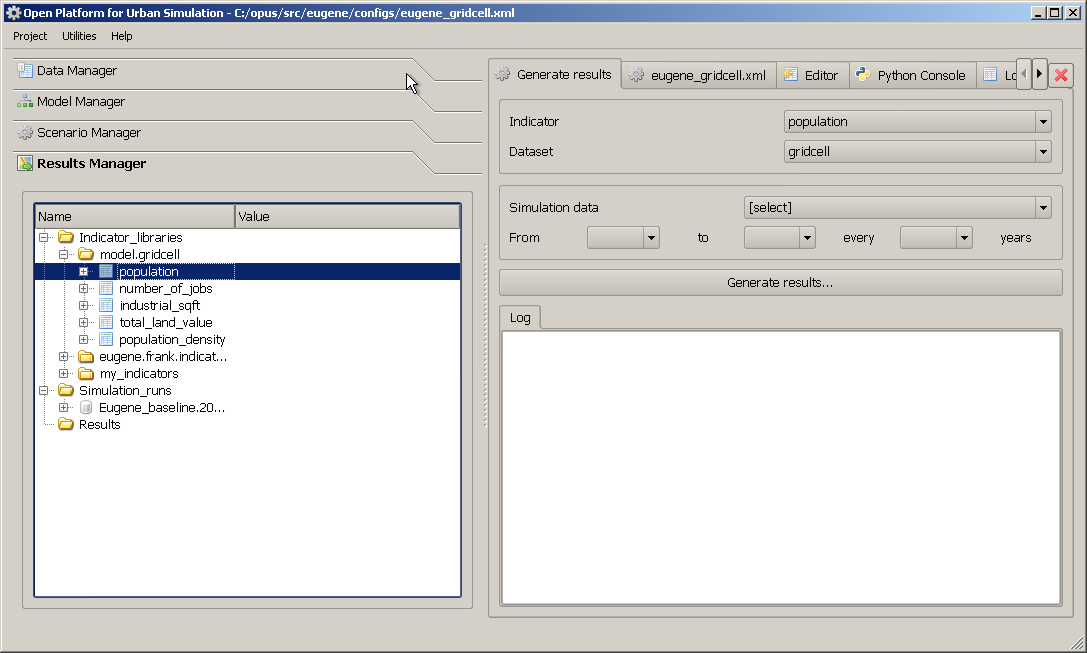
\includegraphics[scale=0.4]{graphics/opus-generate-indicator.png}
\end{center}
\caption{Generating an Indicator in the Results Manager}
\label{fig:opus-generate-indicator}
\end{figure}

You will need to click the \verb#Simulation data# button and then select the simulation results you want to use.  Notice that the name of the scenario contains a date and time when the run was started.  Once you click on the \verb#Generate results# button, the indicator is computed.  A message is printed to the log, below the button, and a new entry will show up in the results node in the Results Manager tab on the left, as shown in Figure \ref{fig:opus-indicator-2}.

\begin{figure}[htp]
\begin{center}
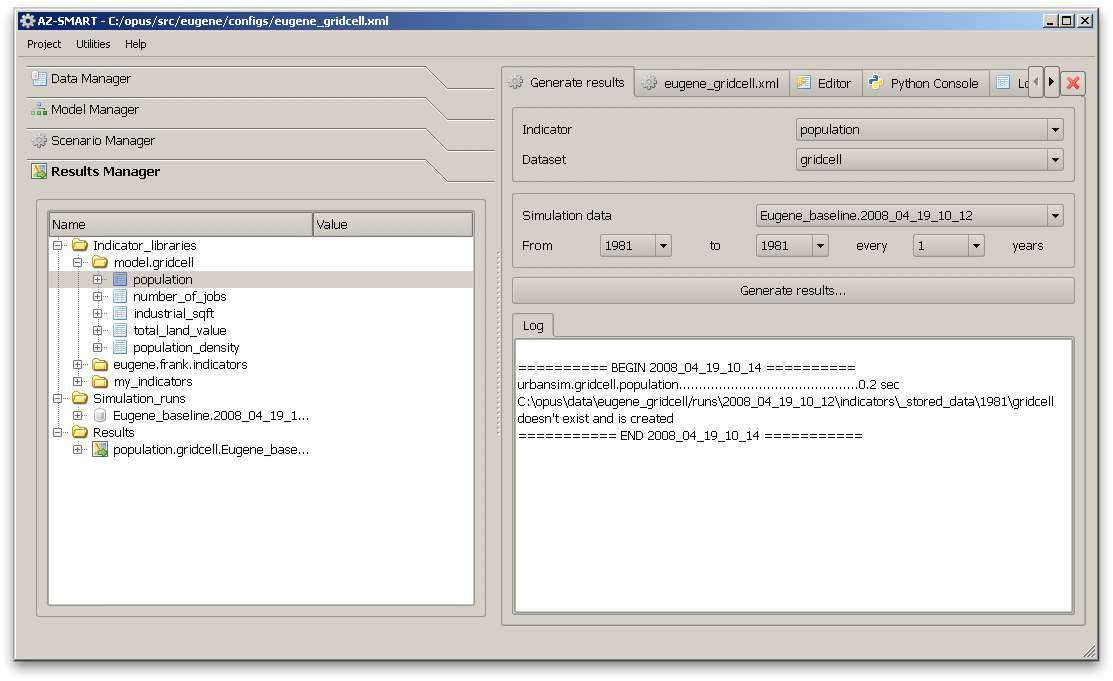
\includegraphics[scale=0.4]{graphics/opus-indicator-2.png}
\end{center}
\caption{Result of Generating an Indicator}
\label{fig:opus-indicator-2}
\end{figure}

Now that an indicator has been computed, its data is available to visualize or export to another application.  The Results Manager currently supports several ways to visualize an indicator, and these will depend on the nature of the indicator.  The menu for this is shown in Figure \ref{fig:opus-indicator-view-1}.  For example, the indicator that has just been computed is population by gridcell.  It is possible to visualize data on a grid using a simple image map, displayed on the right hand window using the Matplotlib Python library.   If you select the Map (Matplotlib) option on the menu, it will generate a map such as the one shown in Figure \ref{fig:opus-indicator-view-2}.

\begin{figure}[htp]
\begin{center}
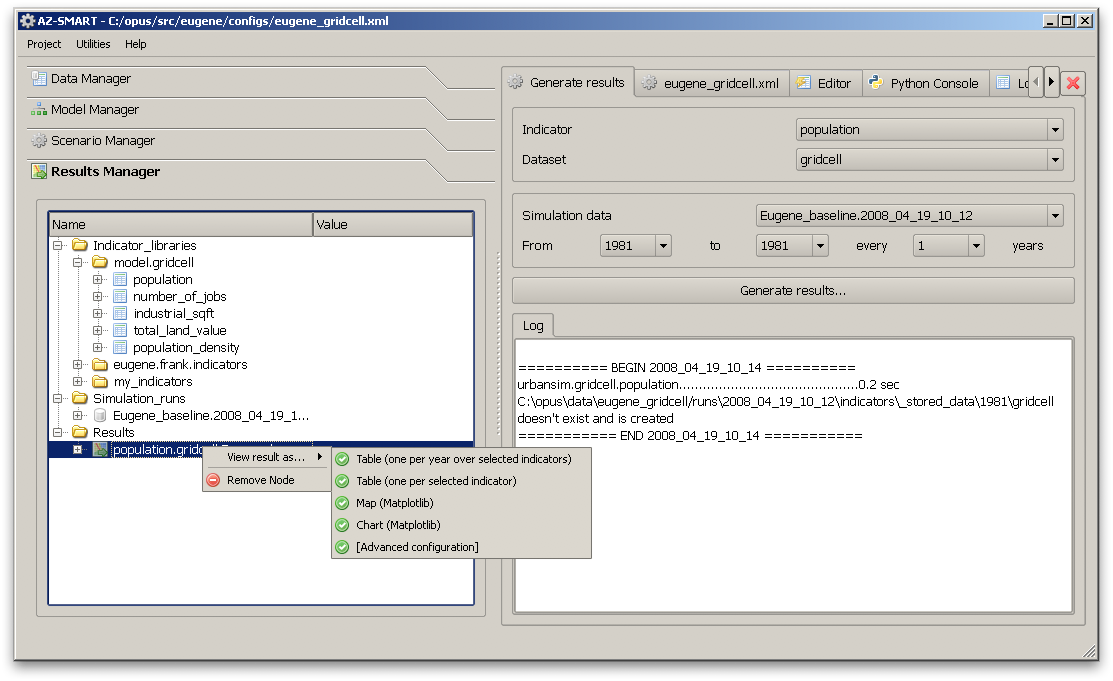
\includegraphics[scale=0.4]{graphics/opus-indicator-view-1.png}
\end{center}
\caption{View Results for an Indicator}
\label{fig:opus-indicator-view-1}
\end{figure}

\begin{figure}[htp]
\begin{center}
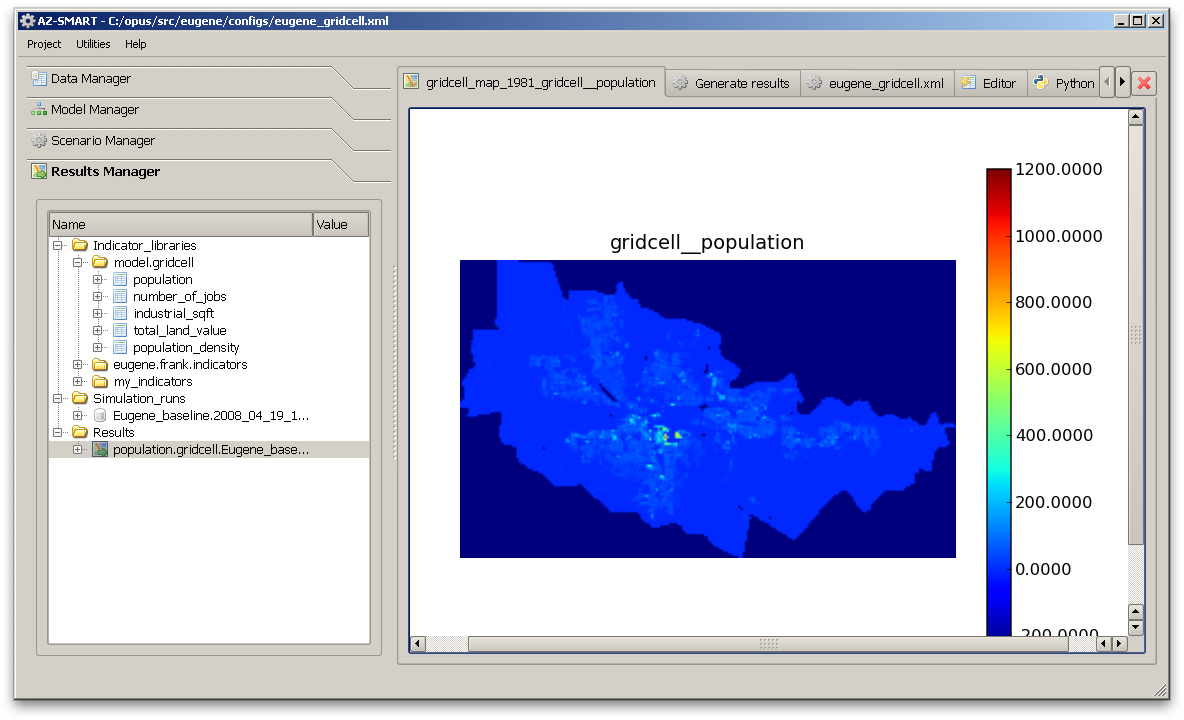
\includegraphics[scale=0.4]{graphics/opus-indicator-view-2.png}
\end{center}
\caption{Matplotlib Map for Population by Gridcell in Eugene-Springfield in 1981}
\label{fig:opus-indicator-view-2}
\end{figure}

The Matplotlib map is not intended to replace GIS-based mapping, which allows far more control and the overlay of other features for visual reference.  It is merely a quick tool to visualize data to get a sense of the spatial patterns in it.  In order to support visualization in a GIS environment such as ArcGIS or QGIS, the results may be exported to a database or geodatabase environment, and the GIS software used to create a more interactive and flexible display of the data.



%%% Local Variables:
%%% mode: latex
%%% TeX-master: "userguide"
%%% End:
